In this paper we introduce translation mechanism of basic concepts employed by Subversion and Git. \emph{Translator} is the server-side implementation of this mechanism.

We use the notation of generalized history to illustrate considered scenarios. The generalized history consists of two layers:
\begin{enumerate}
	\item Subversion history layer. See diagram \ref{svn_layer}.
	\begin{figure}[!h]
	\label{svn_layer}
	\centering
	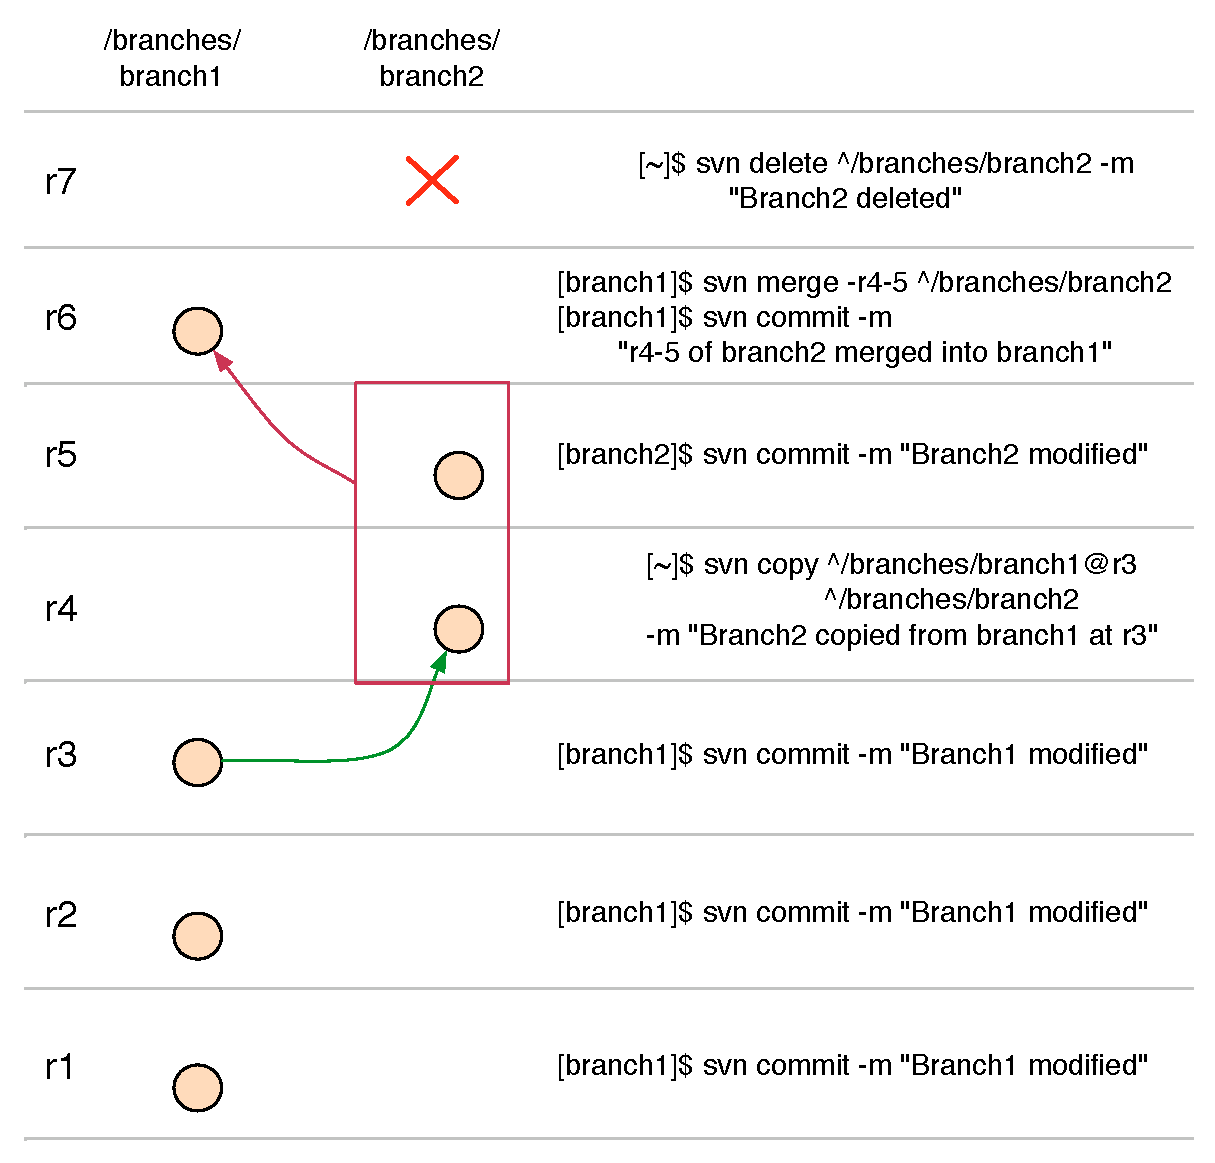
\includegraphics[width=\linewidth]{img/legend/svn_layer.pdf}
	\caption{Subversion history layer.}
	\end{figure}

	\newpage
	\item Git history layer. See diagram \ref{git_layer}.
	\begin{figure}[!h]
	\label{git_layer}
	\centering
	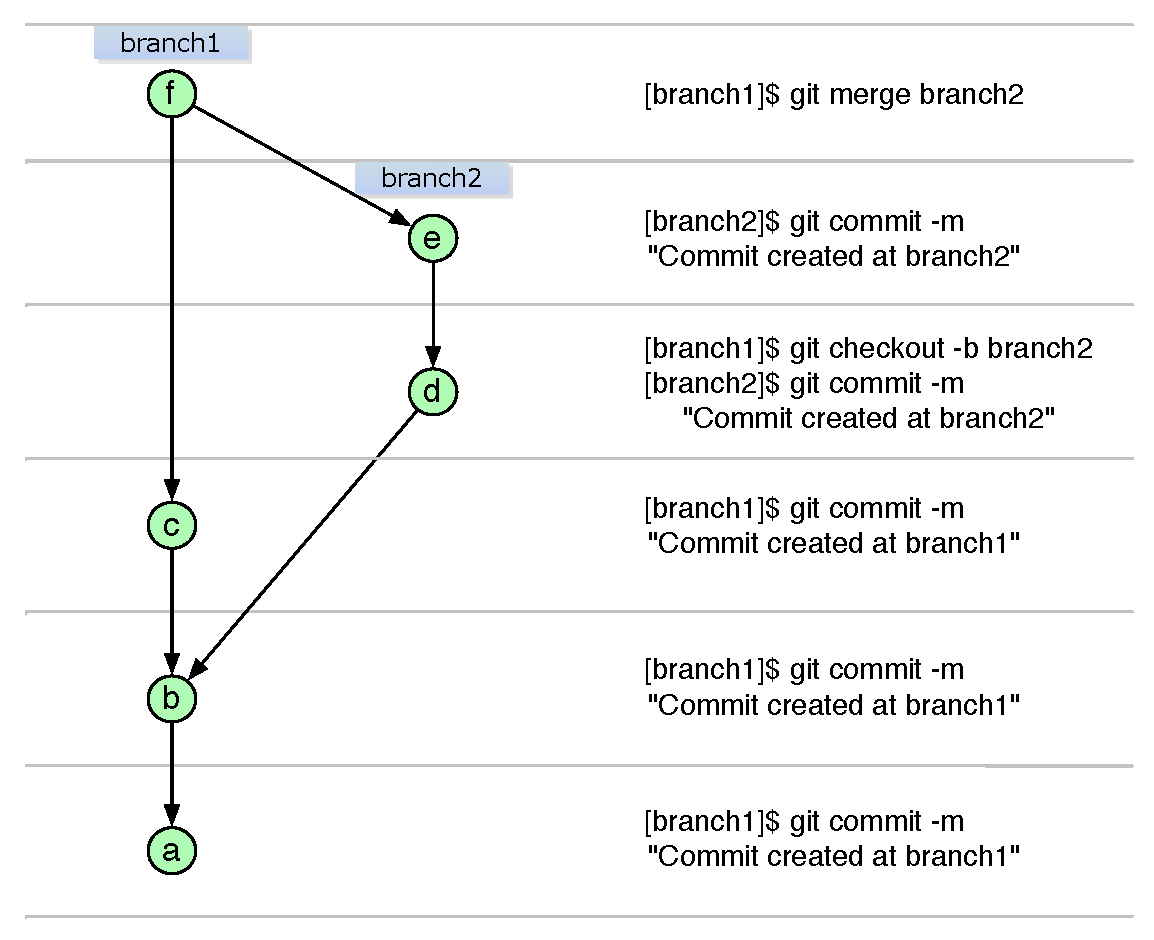
\includegraphics[width=\linewidth]{img/legend/git_layer.pdf}
	\caption{Git history layer.}
	\end{figure}
\end{enumerate}

\newpage
These two layer joined together to put Git commits on top of corresponding SVN revisions as depicted at diagram \ref{both_layers}.
\begin{figure}[!h]
\label{both_layers}
\centering
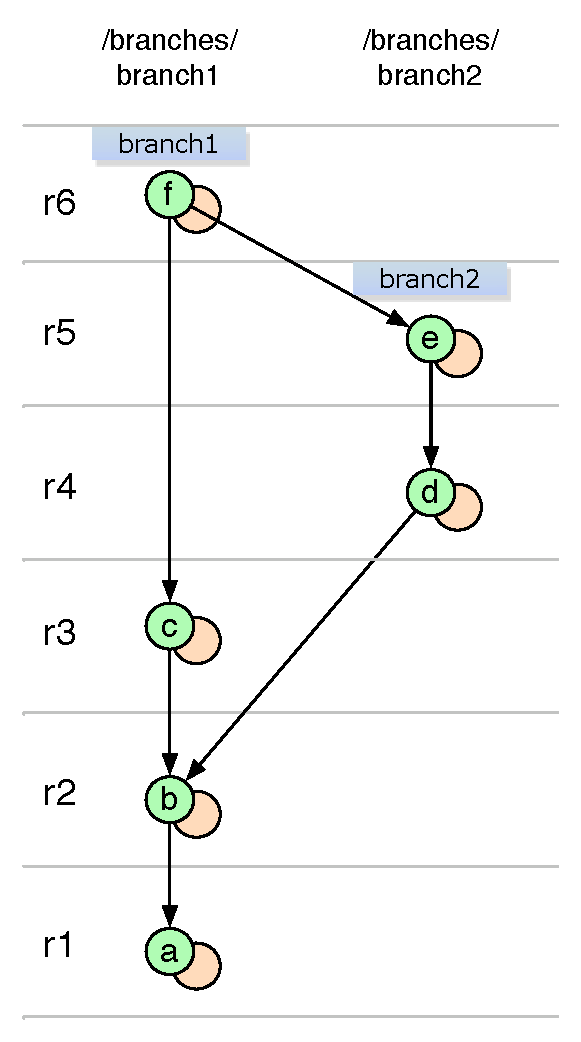
\includegraphics[width=7.0cm]{img/legend/generalized_history.pdf}
\caption{Generalized history.}
\end{figure}